\uuid{cdy7}
\exo7id{5551}
\titre{exo7 5551}
\auteur{rouget}
\organisation{exo7}
\datecreate{2010-07-15}
\isIndication{false}
\isCorrection{true}
\chapitre{Conique}
\sousChapitre{Hyperbole}
\module{Géométrie}
\niveau{L2}
\difficulte{}

\contenu{
\texte{
Soit $(\mathcal{H})$ une hyperbole équilatère de centre $O$ et $P$ et $Q$ deux points de
$(\mathcal{H})$ symétriques par rapport à $O$. Montrer que le cercle de centre $P$ et de rayon $PQ$ recoupe
$(\mathcal{H})$ en trois points formant un triangle équilatéral de centre $P$.
}
\reponse{
On choisit un repère orthonormé dans lequel $P$ a pour coordonnées $(a,b)$, $a>0$, $b>0$ et l'hyperbole $\mathcal{H}$ a pour équation $xy=ab$.
Le cercle $\mathcal{C}$ de centre $P$ et de rayon $PQ$ admet pour représentation paramétrique 
$\left\{\begin{array}{l}
x=a+2\sqrt{a^2+b^2}\cos t\\
y=b+2\sqrt{a^2+b^2}\sin t
\end{array}
\right.$, $t\in\Rr$. Soit donc $M\left(a+2\sqrt{a^2+b^2}\cos t,b+2\sqrt{a^2+b^2}\sin t\right)$ un point de $\mathcal{C}$.

\begin{align*}\ensuremath
M\in\mathcal{C}&\Leftrightarrow(a+2\sqrt{a^2+b^2}\cos t)(b+2\sqrt{a^2+b^2}\sin t)=ab\\
 &\Leftrightarrow2\sqrt{a^2+b^2}(b\cos t+a\sin t)+4(a^2+b^2)\cos t\sin t=0\\
  &\Leftrightarrow2(a^2+b^2)\left(\frac{b}{\sqrt{a^2+b^2}}\cos t+\frac{a}{\sqrt{a^2+b^2}}\sin t+\sin(2t)=0\right)\\
  &\Leftrightarrow\sin(2t)+\sin(t+t_0)+0\;\text{où}\;\cos(t_0)=\frac{a}{\sqrt{a^2+b^2}}\;\text{et}\;\sin(t_0)=\frac{b}{\sqrt{a^2+b^2}}\\
  &\Leftrightarrow\exists k\in\Zz/\;2t=-t-t_0+2k\pi\;\text{ou}\;\exists k\in\Zz/\;2t=\pi+t+t_0+2k\pi\\
  &\Leftrightarrow\exists k\in\Zz/\;t=-\frac{t_0}{3}+\frac{2k\pi}{3}\;\text{ou}\;\exists k\in\Zz/\;t=\pi+t_0+2k\pi.
\end{align*}
$t=\pi+t_0+2k\pi$ fournit le point de coordonnées $(-a,-b)$ c'est-à-dire le point $Q$. Sinon, on obtient trois autres points les points $M\left(-\frac{t_0}{3}\right)$, $M\left(-\frac{t_0}{3}+\frac{2\pi}{3}\right)$ et $M\left(-\frac{t_0}{3}+\frac{4\pi}{3}\right)$. On note $A$, $B$ et $C$ ces trois points. Puisque ces trois points sont sur un cercle de centre $P$ et que $\left(\overrightarrow{PA},\overrightarrow{PB}\right)=\left(\overrightarrow{PB},\overrightarrow{PC}\right)=\left(\overrightarrow{PC},\overrightarrow{PA}\right)=\frac{2\pi}{3}$, le triangle $ABC$ est équilatéral.

$$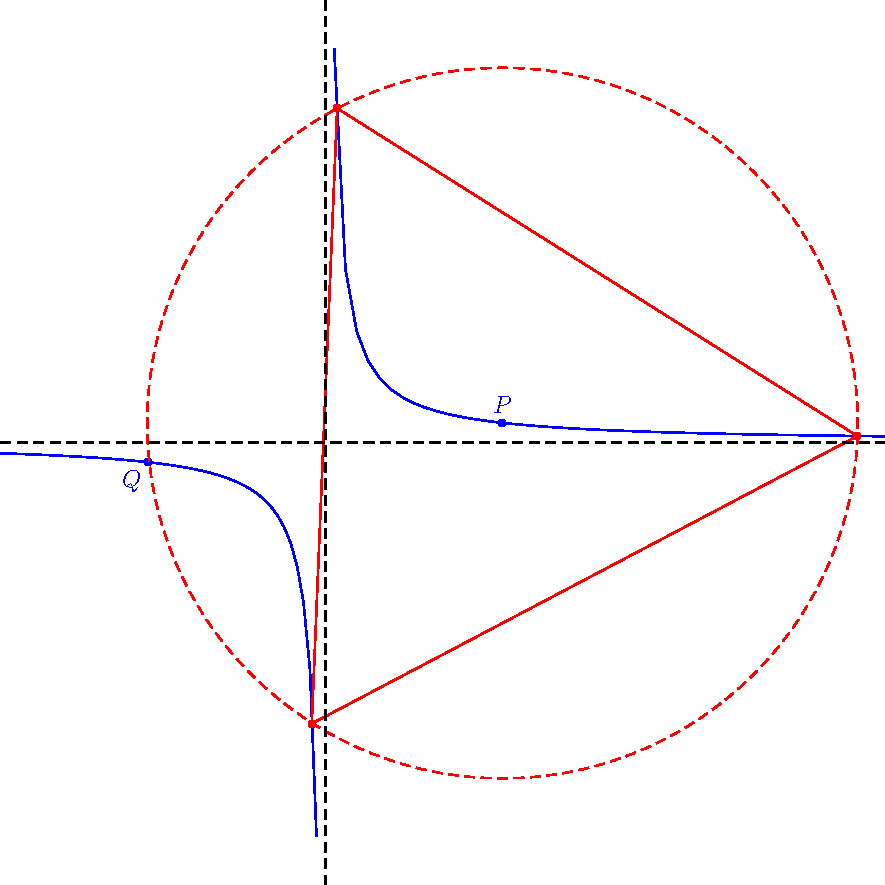
\includegraphics{../images/img005551-1}$$
}
}
